\documentclass[11pt]{article}
\pagestyle{empty}
\usepackage{color}
\usepackage{fancyhdr}
\usepackage{lastpage}
\pagestyle{fancy}
\renewcommand{\headrulewidth}{0pt}
\cfoot[R]{\thepage~of~\pageref{LastPage}}
\addtolength{\oddsidemargin}{-.875in}
\addtolength{\evensidemargin}{-.875in}
\addtolength{\textwidth}{1.75in}
\addtolength{\topmargin}{-.875in}
\addtolength{\textheight}{1.75in}
\usepackage{graphicx}
\graphicspath{ {/} }
\usepackage{amsfonts}
\usepackage{amsmath}
\usepackage{subcaption}
\usepackage{minted}

\title{Cryptocurrencies and Decentralized Ledgers Homework 3}
\author{quentin.mcgaw (qm301)}
\date{November 2017}

\begin{document}

\maketitle

\begin{enumerate}

\item \textbf{\textcolor{blue}{Idioms of use: Consider the transaction graph in the figure below.}}
\begin{center}
  \makebox[\textwidth]{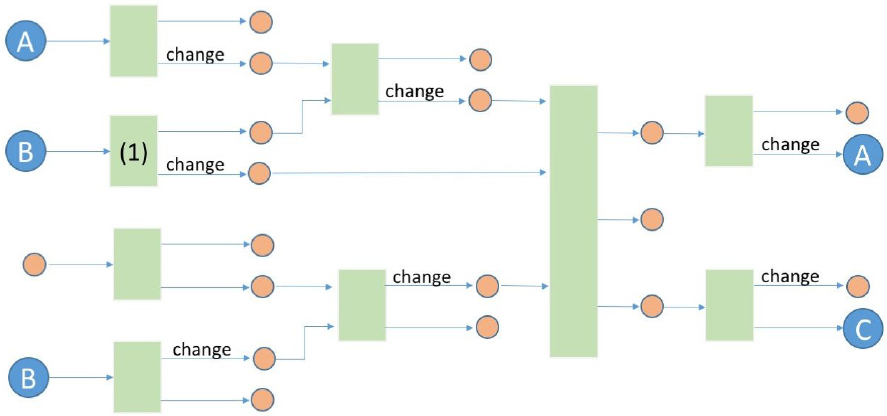
\includegraphics[width=\textwidth]{diagram0.png}}
\end{center}

\begin{figure}[h!]
\centering
\begin{minipage}{.3\textwidth}
  \centering
  
\includegraphics[width=.4\linewidth]{diagram0_transaction.png}
  \captionof{figure}{Transaction}
\end{minipage}
\begin{minipage}{.3\textwidth}
  \centering
  
\includegraphics[width=.4\linewidth]{diagram0_freshaddress.png}
  \captionof{figure}{Fresh address}
\end{minipage}
\begin{minipage}{.3\textwidth}
  \centering
  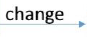
\includegraphics[width=.4\linewidth]{diagram0_change.png}
  \captionof{figure}{The end node of this change edge is the change address for the transaction (identified by heuristics). Note that not every transaction has an identified change address.}
\end{minipage}
\end{figure}

\begin{figure}[h!]
\centering
\begin{minipage}{.3\textwidth}
  \centering
  
\includegraphics[width=.4\linewidth]{diagram0_entityaddress_alice.png}
  \captionof{figure}{Addresses controlled by the entity Alice}
\end{minipage}
\hspace{6pt}
\begin{minipage}{.3\textwidth}
  \centering
  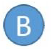
\includegraphics[width=.4\linewidth]{diagram0_entityaddress_bob.png}
  \captionof{figure}{Addresses controlled by the entity Bob}
\end{minipage}
\hspace{6pt}
\begin{minipage}{.3\textwidth}
  \centering
  
\includegraphics[width=.4\linewidth]{diagram0_entityaddress_carol.png}
  \captionof{figure}{Addresses controlled by the entity Carol}
\end{minipage}
\end{figure}
    \begin{enumerate}
    \item \textbf{\textcolor{blue}{Can an observer identify who was paid by Bob in the transaction marked (1)? Explain how or explain why they cannot be identified with certainty.}}
        The oldest transaction involving Alice consists in one input from an address owned by Alice to two outputs:
        \begin{itemize}
            \item A change output, hence going back to Alice in her fresh address that we call $A_1$
            \item Another output, which goes to an unknown fresh address
        \end{itemize}
        In the transaction $1$, there is one input originating from Bob and two outputs:
        \begin{itemize}
            \item A change output, hence going back to Bob in his fresh address that we call $B_1$
            \item Another output to a fresh address, let say $X$, which serves as one of the TWO inputs of a transaction $T_2$, where the second input is provided by $A_1$ (or Alice).
        \end{itemize}
        This transaction $T_2$ has then two outputs:
        \begin{itemize}
            \item A change output, hence going back to Alice in her fresh address that we call $A_2$
            \item Another output, which goes to an unknown fresh address
        \end{itemize}
        As Alice plugs her change address $A_1$ to form one of the two inputs in $T_2$, and also receives the change output of $T_2$, it is very likely Bob previously paid Alice. Alice is likely using the fresh address $X$ on which Bob paid her to form the transaction $T_2$ to pay an unknown entity.
        \\ It is thus likely that Bob paid Alice. However, this could also be another scenario. For example, both Alice and Bob would have to pay a certain entity in this one transaction $T_2$.
    \item \textbf{\textcolor{blue}{Can an observer identity who paid Carol? Explain how or explain why she cannot be identified with certainty.}}
        \\ It is likely that Bob paid Carol.
        \\ The transaction paying Carol, that we name $T_C$ has also another change output, which can be to Alice, Bob or an unknown entity.
        \\ The address serving the input to $T_C$ is a fresh address that we name $X$, receiving funds from a complex transaction, that we name $T_Z$.
        \\ Tracing back from right to left, the transaction $T_Z$ has three inputs likely to be from Alice (top), Bob (middle) and Bob (bottom). The addresses receiving funds from $T_Z$ are likely to belong to the following:
        \begin{itemize}
            \item Top: Alice, because the change is going to Alice
            \item Middle: Unknown
            \item Bottom ($X$): Bob, because a change edge follows $T_C$ and because the only other entity sending all its funds to $T_Z$ is Bob. It is thus likely this change output from $T_C$ is going back to a fresh address owned by Bob.
        \end{itemize}
        Is is thus likely that Carol was paid by Bob.
        \\ On the other hand, there is still many possibilities which are more unlikely, as the bottom input of $T_Z$ could be from an unknown entity instead of Bob for example.
    \end{enumerate}
    
    
\item \textbf{\textcolor{blue}{Mix aggregation: Suppose Bitcoin was changed such that transactions can have at most two inputs and two outputs (this is the case in Zerocash, for example). Alice, Bob, and Carol each have a single UTXO worth 1 BTC. They want to mix their coins among the three of them (without a trusted server) so that three output UTXOs are worth 1 BTC each and they are perfectly shuffled: all six (3!) permutations are equally likely. They decide to do the following: Alice and Bob post a transaction with their two bitcoins as input and two fresh addresses, X and Y, as outputs, each holding 1 BTC. Alice controls one address and Bob controls the other, but an observer cannot tell which is which. Suppose X is listed as the first output in this transaction. Next, Carol and the owner of X post a similar transaction: Carol's coin and the coin X are the inputs, and two fresh addresses W and Z are the outputs, each holding 1 BTC. Carol controls one address and the owner of X controls the other. As before, an observer cannot tell which is which. They use Y,Z,W as the final shuffled coins.}}
\begin{center}
  \makebox[\textwidth]{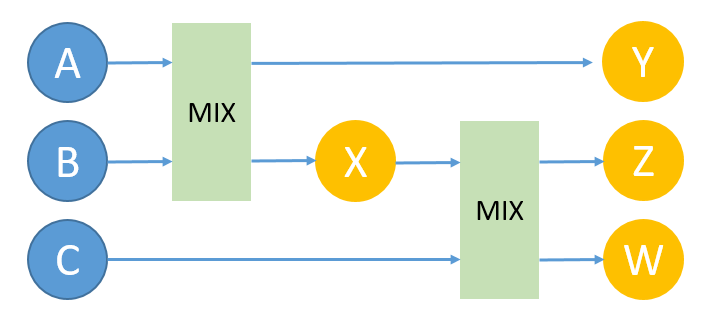
\includegraphics[width=\textwidth]{diagram1.png}}
\end{center}
    \begin{enumerate}
        \item \textbf{\textcolor{blue}{What are the anonymity sets for the addresses Y, Z, and W?}}
            \begin{itemize}
                \item Y: \{A, B\}
                \item Z: \{A, B, C\}
                \item W: \{A, B, C\}
            \end{itemize}
            
        \item \textbf{\textcolor{blue}{Assuming that each mix independently assigns equal probability to both outcomes, what is the probability that Alice controls address W? What is the probability that Carol controls W?}}
            \\ $P(\text{Alice controls address W}) = P(\text{Alice controls address X}) \times 0.5 = 0.5 \times 0.5 = 0.25$
            \\ $P(\text{Carol controls address W}) = 0.5$
            
        \item \textbf{\textcolor{blue}{Suppose at a later time it is revealed that Bob controls W. What else does this reveal?}}
            \\ If Bob controls W, then:
            \begin{itemize}
                \item Bob also controls X and therefore Alice controls Y.
                \item Carol controls Z.
            \end{itemize}
            
        \item \textbf{\textcolor{blue}{Clearly this mix is inadequate as the six possible permutations are not equally likely. By adding one transaction to the mix, can you help Alice, Bob, and Carol design a better mix so that all six (3!) permutations are equally likely to an outside observer?}}
            \\ The following diagram makes all 6 permutations possible to happen.
            \begin{center}
              \makebox[\textwidth]{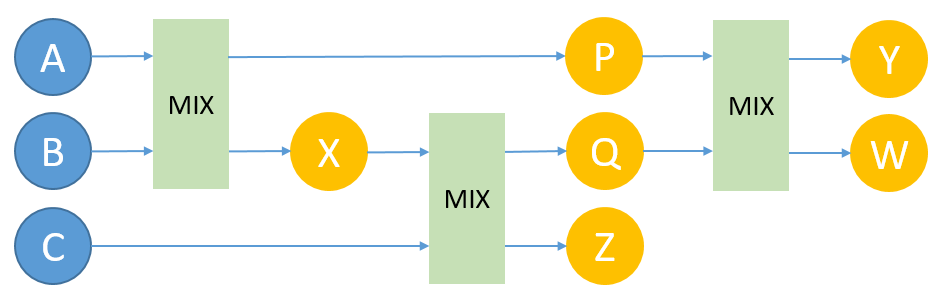
\includegraphics[width=400pt]{diagram2.png}}
            \end{center}
    \end{enumerate}


\item \textbf{\textcolor{blue}{Ethereum data structures. Ethereum replaces Bitcoin's standard Merkle trees with "Merkle Patricia trees", also known as radix tries, prefix trees, tries, and several other names. Ethereum's specific implementation maps keys (or paths) of 256 bits to values of 256 bits. The tree allows three types of nodes, each represented by a 256-bit identifier:
\begin{itemize}
    \item empty nodes, represented as all zeroes (elided from the diagram below)
    \item diverge nodes, which are represented by the hash of a 17-member array. The first 16 items in the array are child node identifiers which contain the hashes of up to 16 child nodes (which will be 0 for empty children). Each child node extends the path of its parent by one nibble (4 bits) of key, defined by its place in the array. This is shown as an edge label in the figure below. The 17th item is a data value (which may be 0) which is mapped to the key representing the path to this node. Internal nodes are represented in blue below, with the child array represented by pointers to child nodes.
    \item kv nodes, which include an arbitrary-length path , plus either the hash of another diverge node or the hash of a data item (making the node a leaf). This path is added to the path built up by this node’s place in the tree. These nodes are shown in pink below. In the following example, 9 keys are present, with 13098a mapped to "c" and 444 to "d": Explain why in the above example there is no label on the arrow coming out of the intermediate node with the path 44.
\end{itemize}
}}
\begin{center}
  \makebox[\textwidth]{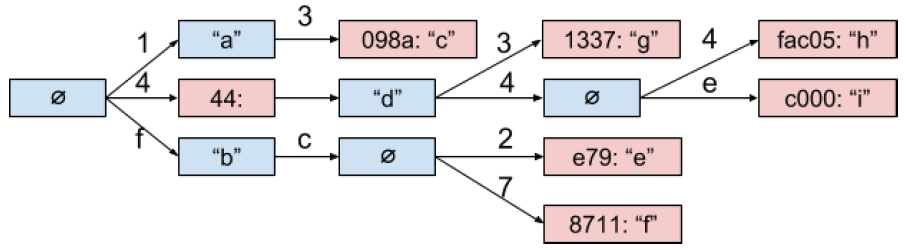
\includegraphics[width=\textwidth]{diagram3.png}}
\end{center}

\begin{enumerate}
    \item \textbf{\textcolor{blue}{Which data would you need to supply for a proof that the key "44431337a" has no data mapped to it? How about the keys "fc" and "1a3098a"?}}
        \begin{itemize}
            \item For "44431337a": The root of the tree and all the arrays of 16 elements up to the depth of the node with key 1337
            \item For "fc": The root of the tree and the arrays of 16 elements following the path f, c
            \item For "1a3098a": The roof the the tree and the arrays of 16 elements for each depth until the kv node with key 098a is reached
        \end{itemize}
    \item \textbf{\textcolor{blue}{Given random keys of arbitrary length, the average-case proof lengths (for both absence and presence) are $O(\log(n))$ for a tree with n elements, as desired. However, constants may vary. Describe a worst-case tree with just k keys that requires proofs of length $O(k)$.}}
        \\ A worst-case tree would be a tree with all the depth levels filled with the maximum possible number of child nodes.
    \item \textbf{\textcolor{blue}{Addresses in Ethereum (for contracts and owned accounts) are 160 bits. Explain why this worst-case proof time is not a serious problem for the tree storing account state.}}
    \item \textbf{\textcolor{blue}{Explain why this does not hold for the trees maintaining the long-term storage for each contract (addressable by 256-bit addresses). How might you write a malicious contract which stores k words in memory and then makes a single write which is expensive as possible?}}
        \\ A malicious contract would write k words such that the maximum number of depth levels in the tree are filled with child nodes. The single extra write would then be the most expensive.
\end{enumerate}

\item \textbf{\textcolor{blue}{Ethereum mixing - Ethereum does not natively support multisig transactions nor transactions with multiple inputs/outputs, so Bitcoin-style mixing approaches like CoinJoin do not work directly. 
\\ Assume Alice, Bob, and Carol have established the following:
\begin{itemize}
    \item Alice has a random byte-array $k_a$ that only she knows
    \item Bob has a random byte-array $k_b$ that only he knows
    \item Carol has a random byte-array $k_c$ that only she knows
    \item $k_a$, $k_b$ and $k_c$ are the same length and as long as needed
    \item $k_a \oplus k_b \oplus k_c = 0$
\end{itemize}
Explain in pseudocode how to implement a mix contract (analogous to CoinJoin) between Alice, Bob, and Carol using these random byte-arrays. Each input account should be able to specify its desired output account, but the output account should be unlinkable to the input account. Recall that every message/transaction sent to the contract costs gas and therefore the account that originated the message/transaction will be known. Your contract should require only one message each from Alice, Bob, and Carol. You should not assume any other infrastructure beyond the Ethereum contract. Make sure to handle the case where one or more participants never send their funds to the mix contract, in which case the other participants should be refunded (at their original address).}}
    \\ Let the destination address of Alice, Bob and Carol be respectively $A_1$, $A_2$ and $A_3$.
    \\ Alice, Bob and Carol respectively one time pad encrypt their respective destination address as follows:
    \begin{itemize}
        \item Enc($A_1$) = $A_1 \oplus k_1$
        \item Enc($A_2$) = $A_2 \oplus k_2$
        \item Enc($A_3$) = $A_3 \oplus k_3$
    \end{itemize}
    The first sender, say Bob, sends Enc($A_2$) with a value to the smart contract
    \\ The smart contract stores Enc($A_2$), Bob's origin address $A_2^\text{origin}$ and the value sent $V_2$. It then waits a certain time for the two other participants to send their ciphertexts and values. If this time is passed, it returns the respective values stored to each participant's origin addresses stored.
    \\ The second participant, say Alice, sends her message. The smart contract stores Enc($A_1$), Alice's origin address $A_1^\text{origin}$ and the value sent $V_1$.
    \\ The third and last participant, say Carol, sends her message. The smart contract stores Enc($A_3$), Carol's origin address $A_3^\text{origin}$ and the value sent $V_3$.
    \\ Given that $k_a \oplus k_b \oplus k_c = 0$, the smart contract deduces $A_1$, $A_2$ and $A_3$ from Enc($A_1$), Enc($A_2$) and Enc($A_3$) and sends the corresponding funds $V_x$ to each addresses $A_1$, $A_2$ and $A_3$
    

\item \textbf{\textcolor{blue}{Ethereum programming - The contract code presented below is an attempt to implement a two-player game (with a wager on the line) of Tic-Tac-Toe. This implementation contains at least 9 bugs which compromise the security of the game. Identify 6 bugs and briefly describe how they might be fixed. Recall that Ethereum initializes all storage to zero. Assume that the function checkGameOver() is correctly implemented and returns true if either player has claimed three squares in a row on the current board.}}
\begin{minted}{c}
contract TicTacToe {
    // game configuration
    address[2] _playerAddress; // address of both players
    uint32 _turnLength; // max time for each turn

    // nonce material used to pick the first player
    bytes32 _p1Commitment;
    uint8 _p2Nonce;

    // game state
    uint8[9] _board; // serialized 3x3 array
    uint8 _currentPlayer; // 0 or 1, indicating whose turn it is
    uint256 _turnDeadline; // deadline for submitting next move

    // Create a new game, challenging a named opponent.
    // The value passed in is the stake which the opponent must match.
    // The challenger commits to its nonce used to determine first mover.
    function TicTacToe(address opponent, uint32 turnLength,
    bytes32 p1Commitment) {
        _playerAddress[0] = msg.sender;
        _playerAddress[1] = opponent;
        _turnLength = turnLength;
        _p1Commitment = p1Commitment;
    }

    // Join a game as the second player.
    function joinGame(uint8 p2Nonce) {
        // only the specified opponent may join
        if (msg.sender != _playerAddress[1])
            throw;
        // must match player 1's stake.
        if (msg.value < this.balance)
            throw;
        _p2Nonce = p2Nonce;
    }

    // Revealing player 1's nonce to choose who goes first.
    function startGame(uint8 p1Nonce) {
        // must open the original commitment
        if (sha3(p1Nonce) != _p1Commitment)
            throw;

        // XOR both nonces and take the last bit to pick the first player
        _currentPlayer = (p1Nonce ^ _p2Nonce) & 0x01;

        // start the clock for the next move
        _turnDeadline = block.number + _turnLength;
    }

    // Submit a move
    function playMove(uint8 squareToPlay) {
        // make sure correct player is submitting a move
        if (msg.sender != _playerAddress[_currentPlayer])
            throw;

        // claim this square for the current player.
        _board[squareToPlay] = _currentPlayer;

        // If the game is won, send the pot to the winner
        if (checkGameOver())
            suicide(msg.sender);

        // Flip the current player
        _currentPlayer ^= 0x1;

        // start the clock for the next move
        _turnDeadline = block.number + _turnLength;
    }

    // Default the game if a player takes too long to submit a move
    function defaultGame() {
        if (block.number > _turnDeadline)
            suicide(msg.sender);
    }
}
\end{minted}

    \begin{itemize}
        \item The function \textbf{TicTacToe} should check that the value sent exists and is strictly positive. A possible fix is to use a modifier as follows:
        \begin{minted}{c}
modifier has_value { if(msg.value > 0) _ }
// ...

function TicTacToe(address opponent, uint32 turnLength, 
    bytes32 p1Commitment) has_value {
    // ...
}
        \end{minted}
        
        \item The function \textbf{TicTacToe} should only be called once per game. A possible fix is:
        \begin{minted}{c}
function TicTacToe(address opponent, uint32 turnLength, 
    bytes32 p1Commitment) has_value {
    if (_playerAddress[0] != address(0)){
        throw;
    }
    // ...
}
        \end{minted}
        
        \item In the function \textbf{TicTacToe}, the balance of the game should be updated by the value sent. A possible fix is:
        \begin{minted}{c}
function TicTacToe(address opponent, uint32 turnLength, 
    bytes32 p1Commitment) has_value {
    if (_playerAddress[0] != address(0)){
        throw;
    }
    if(this.balance == 0) {
        this.balance += msg.value;
    }
    // ...
}
        \end{minted}
        
        \item The function \textbf{joinGame} should check that the value sent exists and is strictly positive. A possible fix is to use a modifier as follows:
        \begin{minted}{c}
modifier has_value { if(msg.value > 0) _ }
// ...

function joinGame(uint8 p2Nonce) has_value {
    // ...
}
        \end{minted}
        
        \item The function \textbf{joinGame} should only be called once per game. A possible fix is:
        \begin{minted}{c}
function joinGame(uint8 p2Nonce) has_value {
    // Check that the second player did not join already
    if (_p2Nonce != 0)
        throw;
    // only the specified opponent may join
    if (msg.sender != _playerAddress[1])
        throw;
    // must match player 1's stake.
    if (msg.value < this.balance)
        throw;
    _p2Nonce = p2Nonce;
}
        \end{minted}
        
        \item In the function \textbf{joinGame}, the balance of the game should be updated by the value sent. A possible fix is:
        \begin{minted}{c}
function joinGame(uint8 p2Nonce) has_value {
    // Check that the second player did not join already
    if (_p2Nonce != 0)
        throw;
    // only the specified opponent may join
    if (msg.sender != _playerAddress[1])
        throw;
    // must match player 1's stake.
    if (msg.value < this.balance)
        throw;
    _p2Nonce = p2Nonce;
    this.balance += msg.value;
}
        \end{minted}
        
        \item The function \textbf{defaultGame} is never called
        
        
    \end{itemize}

\end{enumerate}

\end{document}